% ===================== LongRCA Bench =====================
\subsection{LongRCA Bench}\label{ds:longrca}
\badgerow{\naturalbadge\ \okbadge\ \lbl{agent + step}\ \lbl{MAS}\ \lbl{long-horizon}\ \lbl{SWE-bench Pro / Terminal-Bench 2 / TravelPlanner / VitaBench / WebArena}}

\begin{identity}
Paper & \emph{LongRCA Bench: Root-Cause Localization in Long-Horizon Agent Trajectories} --- Zhang, Feng, Pei et al.\ (CNIC CAS, UCAS, Chongqing Univ., ICT CAS, SMU, Tongyi Lab, Tsinghua), arXiv:2608.15242 (v4, Sep 2026, no venue) \cite{longrca2026}\\
Links & \href{https://huggingface.co/datasets/CLoud5-real/longrca-bench}{HF \code{CLoud5-real/longrca-bench}} \textperiodcentered\ \href{https://longrca-bench.github.io/}{project page + leaderboard} (no separate code repository found)\\
License & none stated on the HF card; paper under the arXiv non-exclusive licence\\
Status & downloaded in full, ungated; 351 MB; \code{data/longrca/} (1,140 full + 200 mini JSON files, 2 parquet files)\\
\end{identity}

\begin{multicols}{2}
\paragraph{Description} LongRCA targets the \emph{long-horizon} regime of the Who\&When task: given a complete failed trajectory (\code{question\_ID} + \code{history}), predict the responsible workflow role (\code{mistake\_agent}) and the earliest decisive root-cause step (\code{mistake\_step}, 0-based); both are scored independently. Median length is 145 steps and the reference root precedes the end of the trajectory by a median of 48 steps. All 1,140 failures are natural, evaluator-confirmed failed attempts freshly generated by the authors with 2026 models (MiniMax-M2.5, Kimi-K2.5, Qwen3.5-Plus) on five sources:
\begin{itemize}
\item \textbf{SWE-bench Pro} (128) and \textbf{Terminal-Bench 2} (42): a custom DiagnostAgent--ActionAgent--JudgeAgent team (diagnosis--execution--verification).
\item \textbf{TravelPlanner} (685): AutoGen MagenticOneGroupChat with manager, stay, transport, food\_attr and verifier agents.
\item \textbf{VitaBench} (108, Chinese-language tool use): Action\_Expert + Computer\_terminal.
\item \textbf{WebArena Verified} (177): Task\_Planner--Action\_Expert (WebSurfer)--Verification\_Expert controller.
\end{itemize}
Normalisation keeps original content, roles and order with stable indices; event granularity therefore differs across sources. \textbf{Annotation}: 22 CS graduate students, calibration on 100 trajectories, then full annotation with the task, the step-indexed history, the evaluator outcome and LLM-written navigation summaries (no root-cause judgement); 30--40 min per trajectory. 294 trajectories were annotated twice or thrice: \textbf{role agreement 66.1\%, exact-step 40.3\%, step $\pm$5 50.3\%}; 38.1\% of pairs differ by $>$20 steps. Disagreements were resolved by two experts; 60 of 1,200 reviewed trajectories were dropped. The root is the earliest step that introduces a decisive, unrepaired error; if a hand-off instruction already contains the error, the instruction step is the root. \textbf{LongRCA-Mini} is a fixed 200-trajectory subset (40 per source, seed 20260821) scored Macro-5; its fidelity to the full set is mean $|\Delta|$ 1.7 pp. No failure taxonomy, only free-text \code{mistake\_reason}.

\paragraph{Metrics and baselines} Agent Acc, Step Acc (exact), Step $\pm$5, Joint Exact / Joint $\pm$5 and Step MAE; invalid outputs count as errors. Full benchmark, DeepSeek-V4-Flash backbone, in \% (paper):

\begin{center}\small
\begin{tabular}{@{}lccc@{}}\toprule
Method & Agent & Step & Step $\pm$5\\\midrule
All-at-Once & 26.2 & 7.6 & 19.9\\
Step-by-Step & 22.2 & 5.3 & 16.9\\
Binary Search & 23.0 & 3.4 & 13.3\\
ECHO & 27.5 & 13.2 & 24.7\\
FALAT & 19.0 & 2.8 & 12.5\\
RCTA (theirs) & \textbf{51.1} & \textbf{24.1} & \textbf{37.4}\\\bottomrule
\end{tabular}
\end{center}
Always predicting each source's majority role already gives 40.3\% Agent Acc. The same six methods reach 30--42\% Step Acc on Who\&When (median 10 steps) but 3--24\% here. On Mini, RCTA scores 60.5\,/\,27.0 (Macro-5 agent\,/\,step) with V4-Flash and up to 64.5\,/\,30.0 with GPT-5.6.

\paragraph{Schema} \code{longrca-full.parquet} (1,140 rows) and \code{longrca-mini.parquet} (200 rows), plus one JSON per trajectory under \code{data/\{full,mini\}/<source>/<source>\_\_NNN.json}. Fields: \code{question\_ID}, \code{history} (list of \{\code{step}, \code{name}, \code{role}, \code{content}\}; \code{role} is \code{assistant} for agent outputs and \code{user} for terminal/tool/evaluator records; hand-off records carry composite names such as \code{DiagnostAgent (-> ActionAgent)}), \code{mistake\_agent}, \code{mistake\_step}, \code{mistake\_reason}. Methods receive only \code{question\_ID} and \code{history}; evaluator feedback (``Run finished: \ldots'') is already inside \code{history}.
\end{multicols}

\paragraph{Statistics} computed from the downloaded data (they match the paper to within rounding).\par\nobreak\vspace{1pt}
\noindent\begin{minipage}[t]{0.60\linewidth}\vspace{0pt}\small
{\footnotesize\fitbox{\begin{tabular}{@{}lrrrrrr@{}}\toprule
 & All & SWE & TB2 & TP & Vita & WA\\\midrule
trajectories: full / mini & 1140 / 200 & 128 / 40 & 42 / 40 & 685 / 40 & 108 / 40 & 177 / 40\\
steps: mean / median & 156 / 145 & 285 / 258 & 272 / 214 & 166 / 165 & 55 / 51 & 59 / 63\\
steps: min -- max & 10 -- 728 & 80 -- 728 & 44 -- 546 & 16 -- 524 & 10 -- 130 & 13 -- 63\\
distinct roles: mean & 5.4 & 7 & 7 & 5.9 & 2 & 4\\
relative root position: mean & 0.53 & 0.25 & 0.29 & 0.60 & 0.45 & 0.56\\
root-to-end distance: median & 47.5 & 184 & 152 & 55 & 24 & 26\\
characters / trajectory: mean & 182\,k & 452\,k & 297\,k & 163\,k & 23\,k & 131\,k\\\bottomrule
\end{tabular}}}

\smallskip Root step (0-based) mean 78.3, median 55.5, max 521; 28.3\% of trajectories have $>$100 steps after the root, 48.6\% $>$50. $\approx$45\,k tokens per trajectory on average (max 1.2\,M characters). The sender of the root step equals the responsible role in 99.2\% of records; 14.9\% of trajectories contain explicit hand-off markers.
\end{minipage}\hfill
\begin{minipage}[t]{0.38\linewidth}\vspace{0pt}
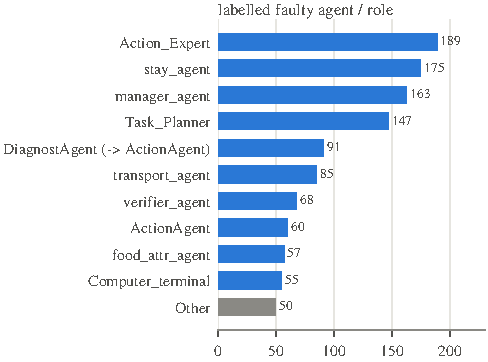
\includegraphics[width=\linewidth]{3_core/longrca/figures/agent.pdf}
\end{minipage}

\paragraph{Example trajectory} \code{webarena\_verified\_\_099} (13 steps, 4 roles, 28.7\,k characters)---the shortest English-language record, chosen for space; a typical trajectory is ten times longer. The Verification\_Expert correctly finds that neither of the two reviews mentions price, but then reports \code{SUCCESS} with an empty list instead of the \code{NOT\_FOUND} status the WebArena RETRIEVE protocol requires.
% auto-generated by scripts/render_traj.py -- do not edit
\trajtask{webarena\_verified\_\_099}{Get name(s) of reviewer(s) who mention price being unfair for the product on the current page}
\begin{trajstep}{0}{Computer\_terminal}{agA}
Get name(s) of reviewer(s) who mention price being unfair for the product on the current page
\end{trajstep}
\begin{trajstep}{1}{Computer\_terminal}{agA}
Orchestration (progress\_packet):\allowbreak{}\newline cycle=\allowbreak{}1
\end{trajstep}
\begin{trajstep}{2}{Task\_Planner}{agB}
Orchestration target:\allowbreak{} Planner\newline This run uses an explicit progress packet handoff. Plan only the next browse step.\par Task prompt:\allowbreak{}\newline You are an autonomous web agent operating in E-commerce Store. Begin from the provided start URLs and work within the current session to complete the task objective.\par \#\# Site Context\par - Platform:\allowbreak{} E-commerce Store\newline - Description:\allowbreak{} An online shopping platform where customers can browse products,\allowbreak{} add items to cart,\allowbreak{} and make purchases.\newline - Authentication:\allowbreak{} You are already logged in as emma.lopez@gmail.com. To re-authenticate,\allowbreak{} use credentials:\allowbreak{} emma.lopez@gmail.com /\allowbreak{} Password.123. If re-authentication fails,\allowbreak{} terminate with PER\newline [...] (2,\allowbreak{}605 chars omitted) [...]\newline this packet turn:\allowbreak{}\newline - Choose exactly one concrete next browse step.\newline - If the recent tactic already failed,\allowbreak{} choose a different action.\newline - Use status fail only when no practical next step remains or the task is clearly blocked.\newline - Do not use markdown fences.
\end{trajstep}
\begin{trajstep}{3}{Task\_Planner}{agB}
Let me analyze the task:\allowbreak{}\par 1. **Task Objective**:\allowbreak{} Get name(s) of reviewer(s) who mention price being unfair for the product on the current page\newline 2. **Start URL**:\allowbreak{} http:\allowbreak{}/\allowbreak{}/\allowbreak{}localhost:\allowbreak{}7770/\allowbreak{}haflinger-men-s-wool-felt-open-back-slippers-beige-550-peat-us-7.html\newline 3. **Task Type**:\allowbreak{} RETRIEVE (we're getting data about reviewers)\par The task is asking me to find reviewers who mentioned that the price is unfair for this product. This requires:\allowbreak{}\newline 1. First,\allowbreak{} navigate to the product page\newline 2. Find the reviews section\newline 3. Look for reviews that mention "price being unfair" or similar\newline 4. Extract the reviewer names from those specific reviews\par Since this is the first cyc\newline [...] (112 chars omitted) [...]\newline king with.\par Let me plan the first browse step:\allowbreak{}\newline - Navigate to the start URL to load the product page\newline - Then inspect the page for a reviews section\newline - Look for reviews that mention the price being unfair\par The first step should be to load the product page.
\end{trajstep}
\begin{trajstep}{4}{Task\_Planner}{agB}
\{"status":\allowbreak{} "act",\allowbreak{} "reason":\allowbreak{} "Starting task to find reviewer names who mention price being unfair. Need to load the product page first.",\allowbreak{} "current\_subgoal":\allowbreak{} "Load product page and find reviews section",\allowbreak{} "instruction\_for\_web\_surfer":\allowbreak{} "Navigate to http:\allowbreak{}/\allowbreak{}/\allowbreak{}localhost:\allowbreak{}7770/\allowbreak{}haflinger-men-s-wool-felt-open-back-slippers-beige-550-peat-us-7.html. Once loaded,\allowbreak{} look for the product reviews section. Identify if there is a Reviews tab,\allowbreak{} link,\allowbreak{} or section on the page. Report back the location of the reviews section and any visible review content.",\allowbreak{} "success\_condition":\allowbreak{} "Product page loaded and reviews section located",\allowbreak{} "facts\_to\_verify":\allowbreak{} ["Product page loads successfully",\allowbreak{} "Reviews section exists on the page"]\}
\end{trajstep}
\begin{trajstep}{5}{Task\_Planner}{agB}
Orchestration target:\allowbreak{} WebSurfer\newline This is an explicit progress packet handoff from Planner to WebSurfer.\newline Do not ask for the task again. Use the packet below and take the minimum number of browser actions needed.\par Task prompt:\allowbreak{}\newline You are an autonomous web agent operating in E-commerce Store. Begin from the provided start URLs and work within the current session to complete the task objective.\par \#\# Site Context\par - Platform:\allowbreak{} E-commerce Store\newline - Description:\allowbreak{} An online shopping platform where customers can browse products,\allowbreak{} add items to cart,\allowbreak{} and make purchases.\newline - Authentication:\allowbreak{} You are already logged in as emma.lopez@gmail.com. To re-authenticate,\allowbreak{} use\newline [...] (2,\allowbreak{}605 chars omitted) [...]\newline ion price being unfair for the product on the current page\newline - Latest critic feedback:\allowbreak{}\newline (none)\newline - Stop condition:\allowbreak{}\newline Product page loaded and reviews section located\par Reply with only direct browser observations,\allowbreak{} concrete evidence,\allowbreak{} or a precise blocking reason.
\end{trajstep}
\begin{trajstep}{6}{Action\_Expert}{agC}
I clicked '2  Reviews'.\par The web browser is open to the page [HAFLINGER Men's Wool Felt Open Back Slippers,\allowbreak{} Beige 550 Peat,\allowbreak{} US:\allowbreak{}7](http:\allowbreak{}/\allowbreak{}/\allowbreak{}localhost:\allowbreak{}7770/\allowbreak{}haflinger-men-s-wool-felt-open-back-slippers-beige-550-peat-us-7.html).\newline The viewport shows 34\% of the webpage,\allowbreak{} and is positioned 48\% down from the top of the page\newline The following text is visible in the viewport:\allowbreak{}\par Skip to the beginning of the images gallery Details\newline Reviews\newline 2Customer Reviews Wonderful!\newline Rating 100\%\newline Nothing.....everyday use.\newline Review by Jay Posted on 4/\allowbreak{}18/\allowbreak{}23 Joe\newline Die Haflinger sind wie beschrieben und erwartet sehr gut\newline Review by Josef Bürger Posted on 4/\allowbreak{}18/\allowbreak{}23 You'\newline [...] (2,\allowbreak{}605 chars omitted) [...]\newline description":\allowbreak{} "",\allowbreak{}\newline "og:\allowbreak{}url":\allowbreak{} "http:\allowbreak{}/\allowbreak{}/\allowbreak{}localhost:\allowbreak{}7770/\allowbreak{}haflinger-men-s-wool-felt-open-back-slippers-beige-550-peat-us-7.html",\allowbreak{}\newline "product:\allowbreak{}price:\allowbreak{}amount":\allowbreak{} "108",\allowbreak{}\newline "product:\allowbreak{}price:\allowbreak{}currency":\allowbreak{} "USD"\newline \}\newline \}\par Here is a screenshot of the page.
\end{trajstep}
\begin{trajstep}{7}{Task\_Planner}{agB}
Orchestration target:\allowbreak{} Critic\newline This run uses an explicit progress packet handoff. Decide whether the task is complete,\allowbreak{} needs one more step,\allowbreak{} or should fail fast.\par Task prompt:\allowbreak{}\newline You are an autonomous web agent operating in E-commerce Store. Begin from the provided start URLs and work within the current session to complete the task objective.\par \#\# Site Context\par - Platform:\allowbreak{} E-commerce Store\newline - Description:\allowbreak{} An online shopping platform where customers can browse products,\allowbreak{} add items to cart,\allowbreak{} and make purchases.\newline - Authentication:\allowbreak{} You are already logged in as emma.lopez@gmail.com. To re-authenticate,\allowbreak{} use credentials:\allowbreak{} emma.lopez@gmail.com /\allowbreak{} Password.123.\newline [...] (2,\allowbreak{}605 chars omitted) [...]\newline t practically reachable,\allowbreak{} recent turns are repeating,\allowbreak{} or the task is blocked.\newline - If status is complete or fail,\allowbreak{} final\_response must be a valid WebArena final JSON object.\newline - If status is continue,\allowbreak{} final\_response must be null.\newline - Do not use markdown fences.
\end{trajstep}
\begin{trajstep}{8}{Verification\_Expert}{agD}
Let me analyze the current state of the task:\allowbreak{}\par 1. **Task Objective**:\allowbreak{} Get name(s) of reviewer(s) who mention price being unfair for the product on the current page\par 2. **Current Progress**:\allowbreak{}\newline - The product page is loaded\newline - Reviews section is visible (2 customer reviews)\newline - The reviews visible are:\allowbreak{}\newline - Review 1:\allowbreak{} "Wonderful!" by Jay - "Nothing.....everyday use."\newline - Review 2:\allowbreak{} "Joe" by Josef Bürger - "Die Haflinger sind wie beschrieben und erwartet sehr gut"\par 3. **Analysis**:\allowbreak{}\newline - Looking at the two reviews visible,\allowbreak{} neither mentions "price being unfair"\newline - Review 1 is positive ("Wonderful!")\newline - Review 2 is in German and says\newline [...] (1,\allowbreak{}225 chars omitted) [...]\newline t might not be showing all review text\par - The metadata confirms only 2 reviews exist,\allowbreak{} with neither mentioning price concerns\par I can confidently conclude that no reviewers mentioned unfair pricing. The task cannot be completed as no such reviews exist.
\end{trajstep}
\begin{faultystep}{9}{Verification\_Expert}{agD}
\{"status":\allowbreak{}"complete",\allowbreak{}"reason":\allowbreak{}"The task asks for reviewer(s) who mention price being unfair. The page shows exactly 2 reviews (visible in both viewport and metadata). Review 1 is by Jay with text 'Nothing.....everyday use.' and Review 2 is by Josef Bürger with text 'Die Haflinger sind wie beschrieben und erwartet sehr gut' (German for 'The Haflingers are as described and expected very good'). Neither review mentions price or indicates the price is unfair. The metadata confirms only these 2 reviews exist for this product. Since no reviewer mentions price being unfair,\allowbreak{} the answer is an empty list.",\allowbreak{}"confirmed\_facts":\allowbreak{}["Product has 2 customer r\newline [...] (151 chars omitted) [...]\newline wie beschrieben und erwartet sehr gut' - no price mention",\allowbreak{}"Neither reviewer mentions price being unfair"],\allowbreak{}"missing\_items":\allowbreak{}[],\allowbreak{}"next\_action\_hint":\allowbreak{}null,\allowbreak{}"final\_response":\allowbreak{}\{"task\_type":\allowbreak{}"RETRIEVE",\allowbreak{}"status":\allowbreak{}"SUCCESS",\allowbreak{}"retrieved\_data":\allowbreak{}[],\allowbreak{}"error\_details":\allowbreak{}null\}\}
\end{faultystep}
\begin{trajstep}{10}{Task\_Planner}{agB}
Orchestration (coordinator\_decision):\allowbreak{}\newline cycle=\allowbreak{}1
\end{trajstep}
\begin{trajstep}{11}{Verification\_Expert}{agD}
Final answer:\allowbreak{}\newline \{"task\_type":\allowbreak{} "RETRIEVE",\allowbreak{} "status":\allowbreak{} "SUCCESS",\allowbreak{} "retrieved\_data":\allowbreak{} [],\allowbreak{} "error\_details":\allowbreak{} null\}
\end{trajstep}
\begin{trajstep}{12}{Computer\_terminal}{agA}
Run finished:\allowbreak{} The task asks for reviewer(s) who mention price being unfair. The page shows exactly 2 reviews (visible in both viewport and metadata). Review 1 is by Jay with text 'Nothing.....everyday use.' and Review 2 is by Josef Bürger with text 'Die Haflinger sind wie beschrieben und erwartet sehr gut' (German for 'The Haflingers are as described and expected very good'). Neither review mentions price or indicates the price is unfair. The metadata confirms only these 2 reviews exist for this product. Since no reviewer mentions price being unfair,\allowbreak{} the answer is an empty list.
\end{trajstep}
\trajannotation{Verification\_Expert}{9}{—}{Verification\_Expert already correctly determined at \#9 that the page has only 2 comments,\allowbreak{} and neither Jay nor Josef Bürger mentioned "price unfair". However,\allowbreak{} it outputs the following in its final\_response:\allowbreak{}\par status:\allowbreak{} "SUCCESS"\newline retrieved\_data:\allowbreak{} []\newline error\_details:\allowbreak{} null\par This violates the WebArena RETRIEVE task specification. For retrieval tasks such as "find the reviewer name",\allowbreak{} if no matching entity exists on the page,\allowbreak{} the correct return should be NOT\_FOUND\_ERROR,\allowbreak{} rather than SUCCESS with an empty list. Therefore,\allowbreak{} the error is not the failure to find the reviewer,\allowbreak{} but the incorrect labeling of the "not found" scenario as successful completion.}{—}{Run finished:\allowbreak{} The task asks for reviewer(s) who mention price being unfair. The page shows exactly 2 reviews (visible in both viewport and metadata). Review 1 is by Jay with text 'Nothing\newline [...] (325 chars omitted) [...]\newline nce no reviewer mentions price being unfair,\allowbreak{} the answer is an empty list.}{\textbf{source\_benchmark}: webarena\_verified; \textbf{step\_indexing}: 0-based,\allowbreak{} field history[].step; \textbf{in\_longrca\_mini}: False}


\paragraph{Notes} (i) An order of magnitude longer than Who\&When (median 145 vs 10 steps, $\approx$45\,k vs 7\,k tokens); SWE-bench Pro and Terminal-Bench 2 trajectories are 4--5$\times$ longer again (up to 450\,k characters). (ii) Source imbalance: TravelPlanner is 60\% of the full set; Mini equalises sources, but the paper insists headline numbers use the full set. (iii) Root position is bimodal: 243 roots lie in the last 10\% of the trajectory (late verifier/planner errors in TravelPlanner and WebArena), while SWE/TB2 roots sit early (relative position 0.25--0.29) followed by hundreds of steps; five roots are at the very last step. (iv) Role quirks: composite hand-off names are themselves reference roles (91 cases) and \code{Computer\_terminal}, an environment relay, is blamed 55 times, so role matching must follow the paper's normalisation; with only 2--7 roles per trajectory, agent accuracy is partly a prior problem. (v) Inter-annotator agreement on the exact step (40.3\%) is itself low, so exact-step accuracy has a limited ceiling. (vi) VitaBench trajectories are in Chinese. No overlap with Who\&When/MAST logs; the paper cites AgentRx's first-unrecoverable-failure definition and TraceElephant.
